\documentclass[a4wide]{report}

\usepackage{amsmath}
\usepackage[a4paper, total={7in, 10.2in}]{geometry}
\usepackage{graphicx}
\usepackage[portuguese]{babel}
\usepackage[utf8]{inputenc}


\begin{document}

\noindent
{\bf Rafael V. Cacilhas  - Relatório 04 (\today)}

\vspace{0.5cm}

\section*{Exercício 1}

\subsection*{a) }
Na figura \ref{solucao} temos o gráfico da solução exata e solução estimada. A análise do gráfico não mostra nenhuma diferença aparente entre as duas soluções, sendo então necessário plotar o gráfico do erro separadamente. Como os métodos mais precisos farão a diferença entre a solução numérica e a solução exata serem ainda menores este gráfico será omitido nas análises posteriores.

Ainda na figura \ref{solucao} temos o erro do método de Euler para N = 365 e N = 730. Como o erro do método é da ordem de h, temos que ao dobrar N o erro cai pela metade, como esperado.


\begin{figure}[!htb]
\centering
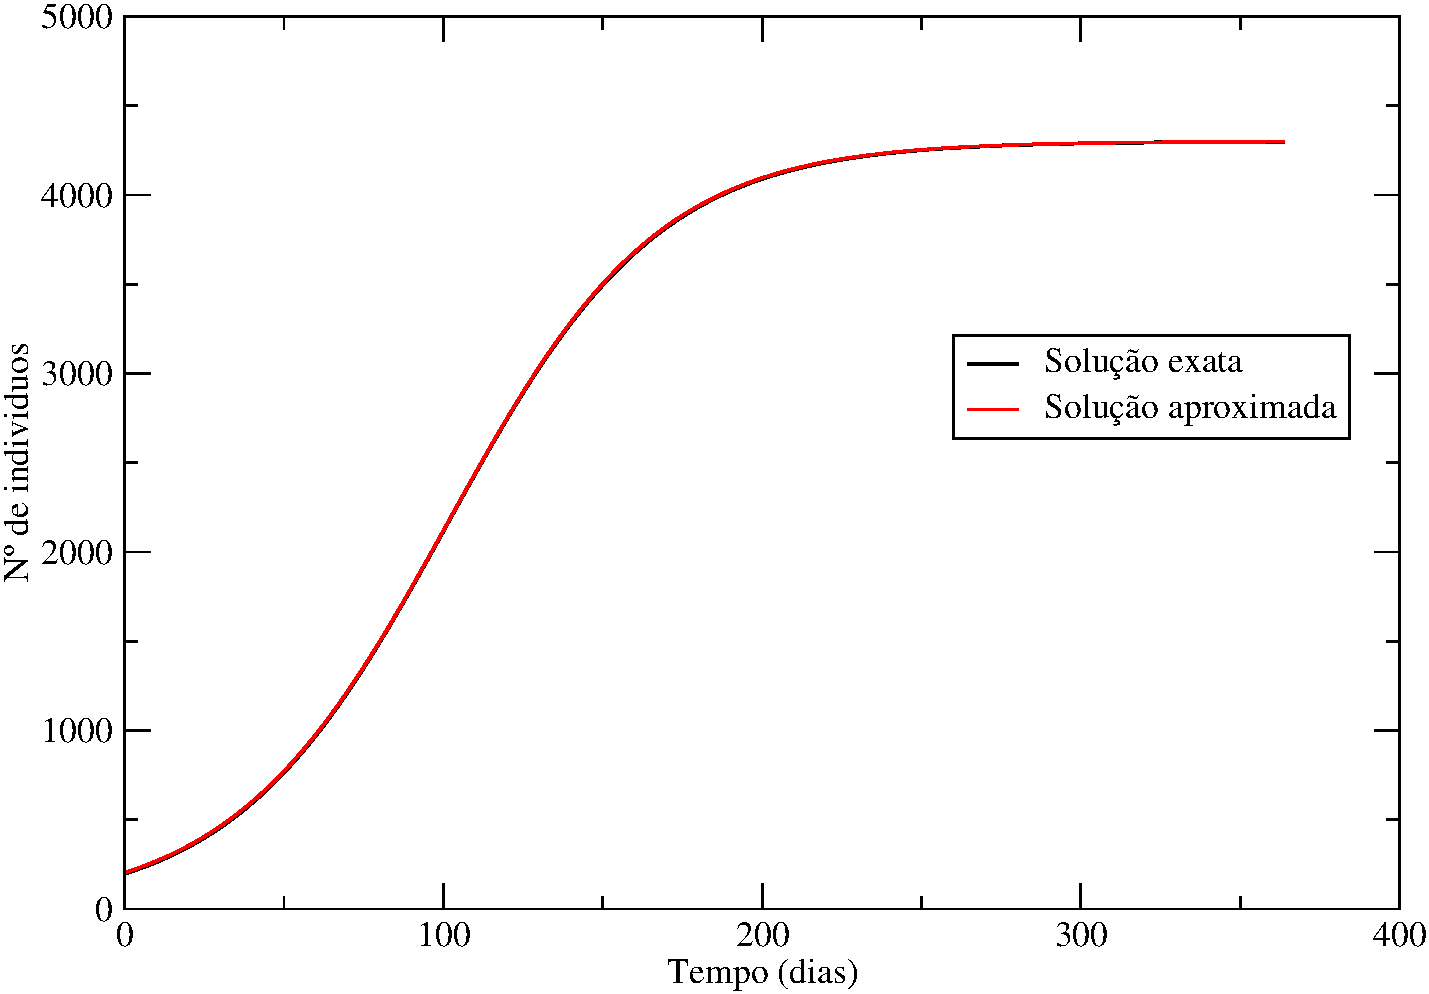
\includegraphics[width=0.447\textwidth]{1a.pdf}
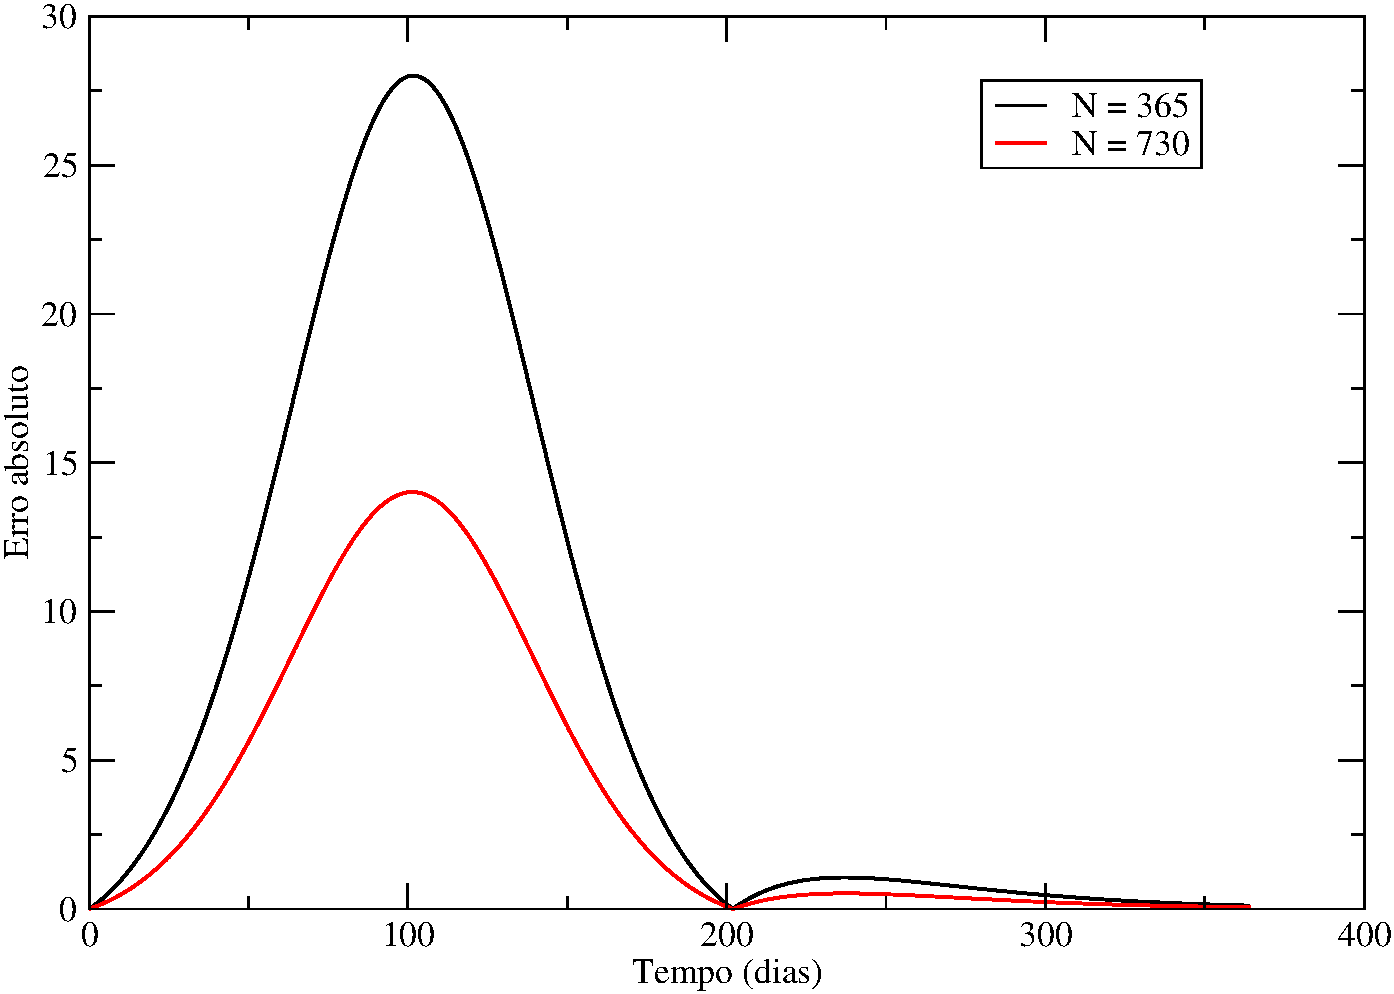
\includegraphics[width=0.447\textwidth]{1erro2.pdf}
\caption{Solução exata e solução numérica em função do tempo (esquerda) e erro absoluto para o método de Euler (direita).}
\label{solucao}
\end{figure}



\subsection*{b)}
 Na figura \ref{erropreditor} temos o erro do método preditor-corretor para dois valores de N. Como o erro é proporcional a $h^2$ temos que dobrar o N faz com o que o erro diminua por 4, como esperado. 

\begin{figure}[!htb]
\centering
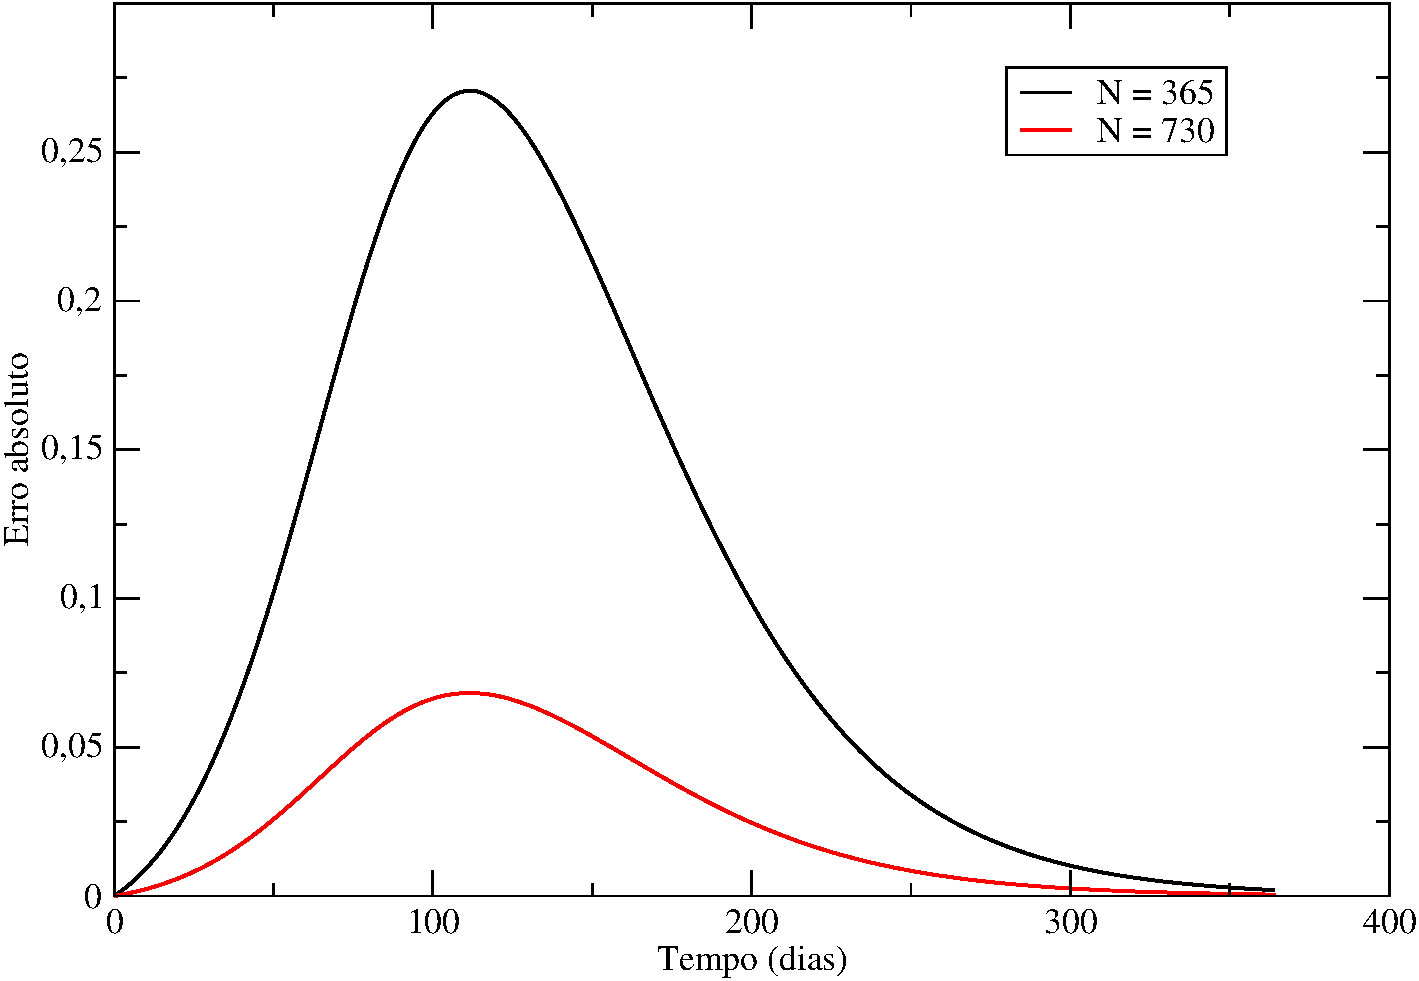
\includegraphics[width=0.447\textwidth]{erroPreditor.pdf}
\caption{Erro absoluto para o método Preditor-Corretor. }
\label{erropreditor}
\end{figure}

Uma comparação direta entre o método de Euler e o método preditor corretor está na figura \ref{erropreditorrk}. Em uma escala linear não é possível diferenciar o erro do método preditor do eixo x, portanto também foi feito o gráfico em escala log-log, onde vemos que os erros do método preditor são por volta de 300 vezes menores. No gráfico log-log há apenas uma regiao onde o método de Euler é menor que o método preditor, o que se deve a um único ponto onde o erro absoluto do método de Euler é nulo. 

\begin{figure}[!htb]
\centering
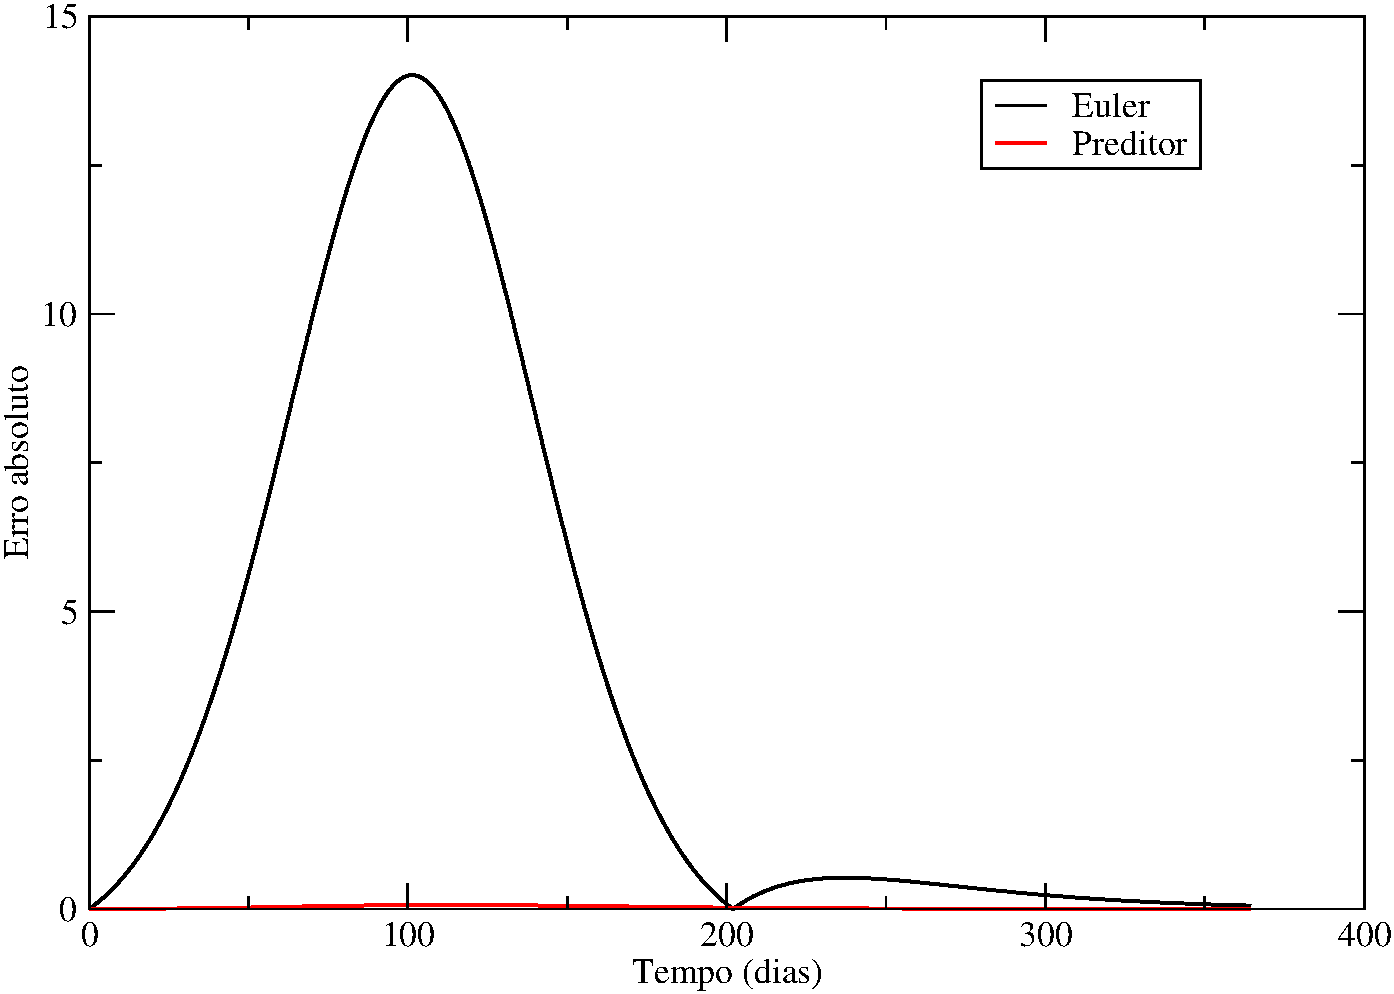
\includegraphics[width=0.447\textwidth]{1erro_preditor.pdf}
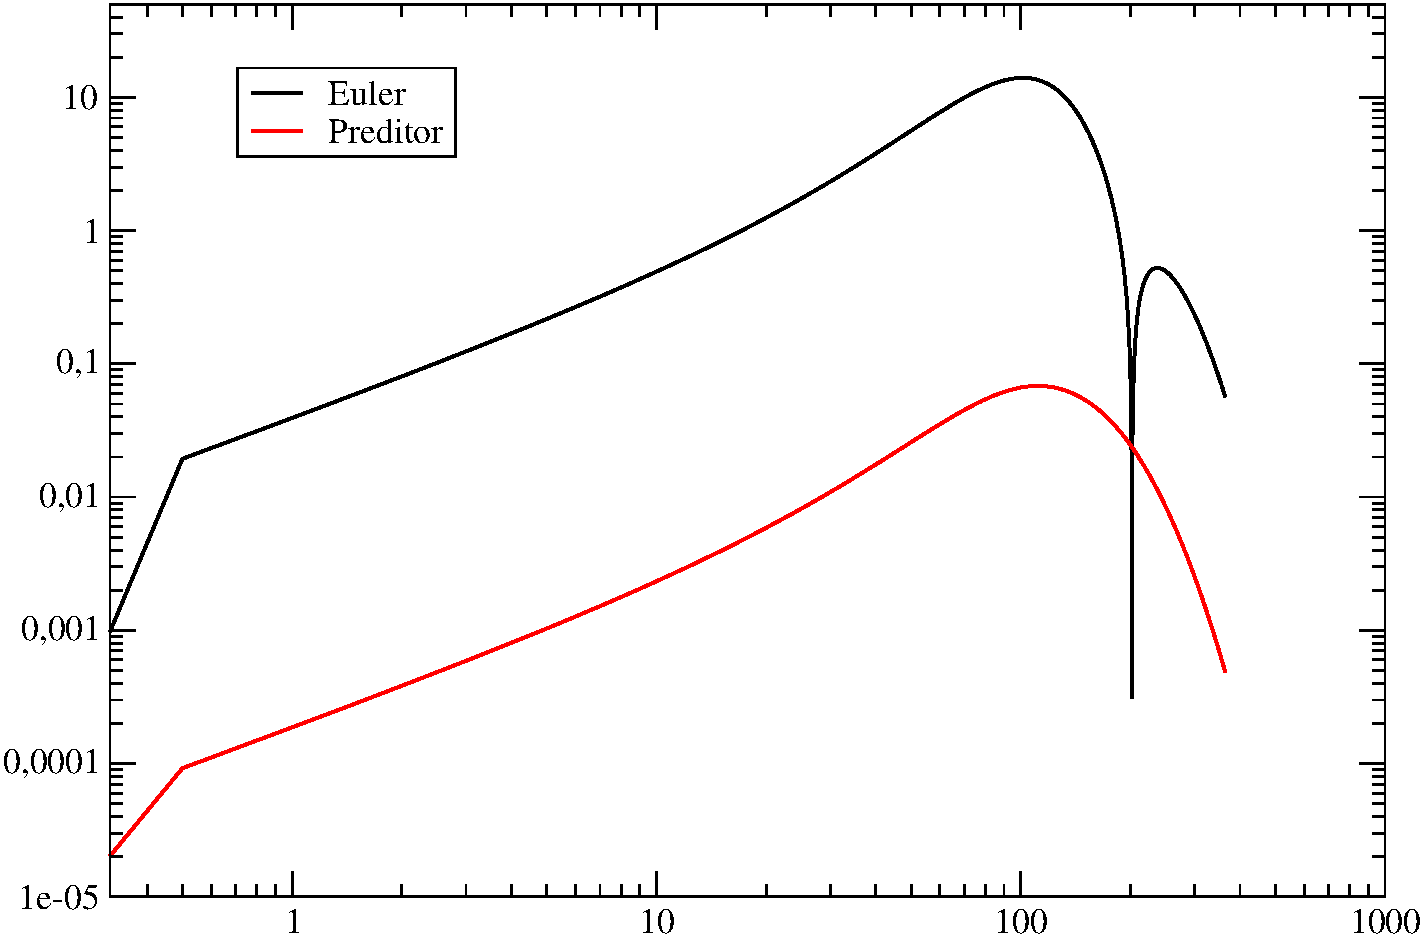
\includegraphics[width=0.447\textwidth]{1erro_euler_preditor_log.pdf}
\caption{Erro absoluto para o método de Euler e preditor-corretor com N = 730. }
\label{erropreditorrk}
\end{figure}


\subsection*{ c) }

Na figura \ref{erroRK} temos o erro absoluto para o método Rouge-Kutta de quarta ordem. Como o erro é da ordem de $h^4$ temos que dobrar o N faz com que o erro diminua em 16 vezes, como esperado.

\begin{figure}[!htb]
\centering
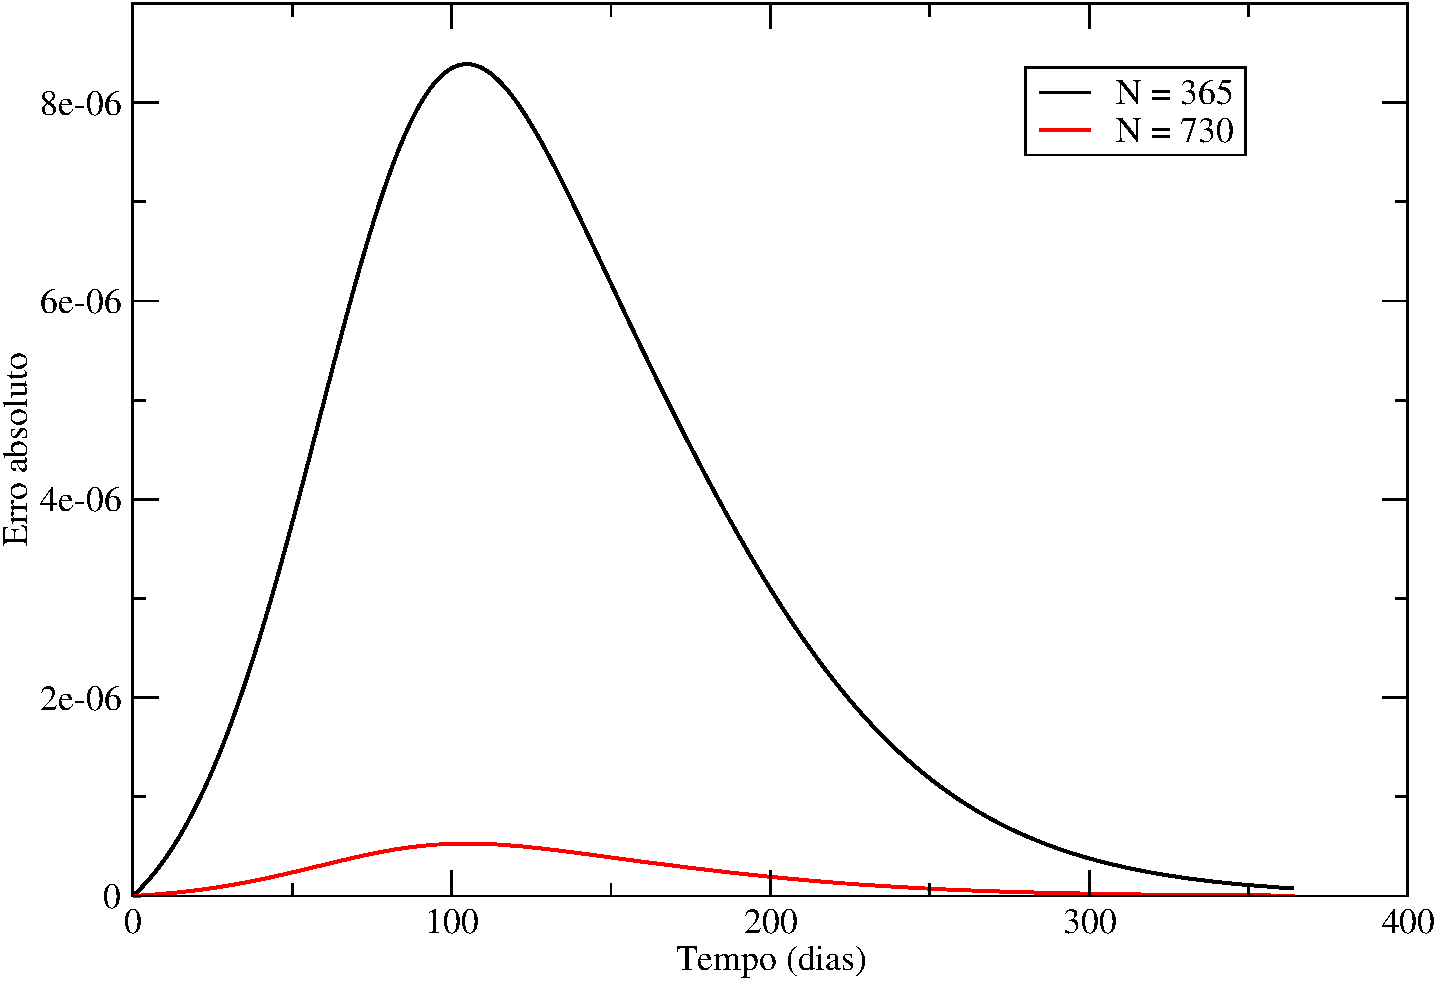
\includegraphics[width=0.447\textwidth]{RKErro.pdf}
\caption{Erro absoluto para o método de Rouge-Kutta. }
\label{erroRK}
\end{figure}


Na figura \ref{errork} temos uma comparação direta entre os métodos de Rouge-Kutta e o método Preditor-Corretor. Vemos que a diferença entre os erros é de 5 ordens de grandeza.




\begin{figure}[!htb]
\centering
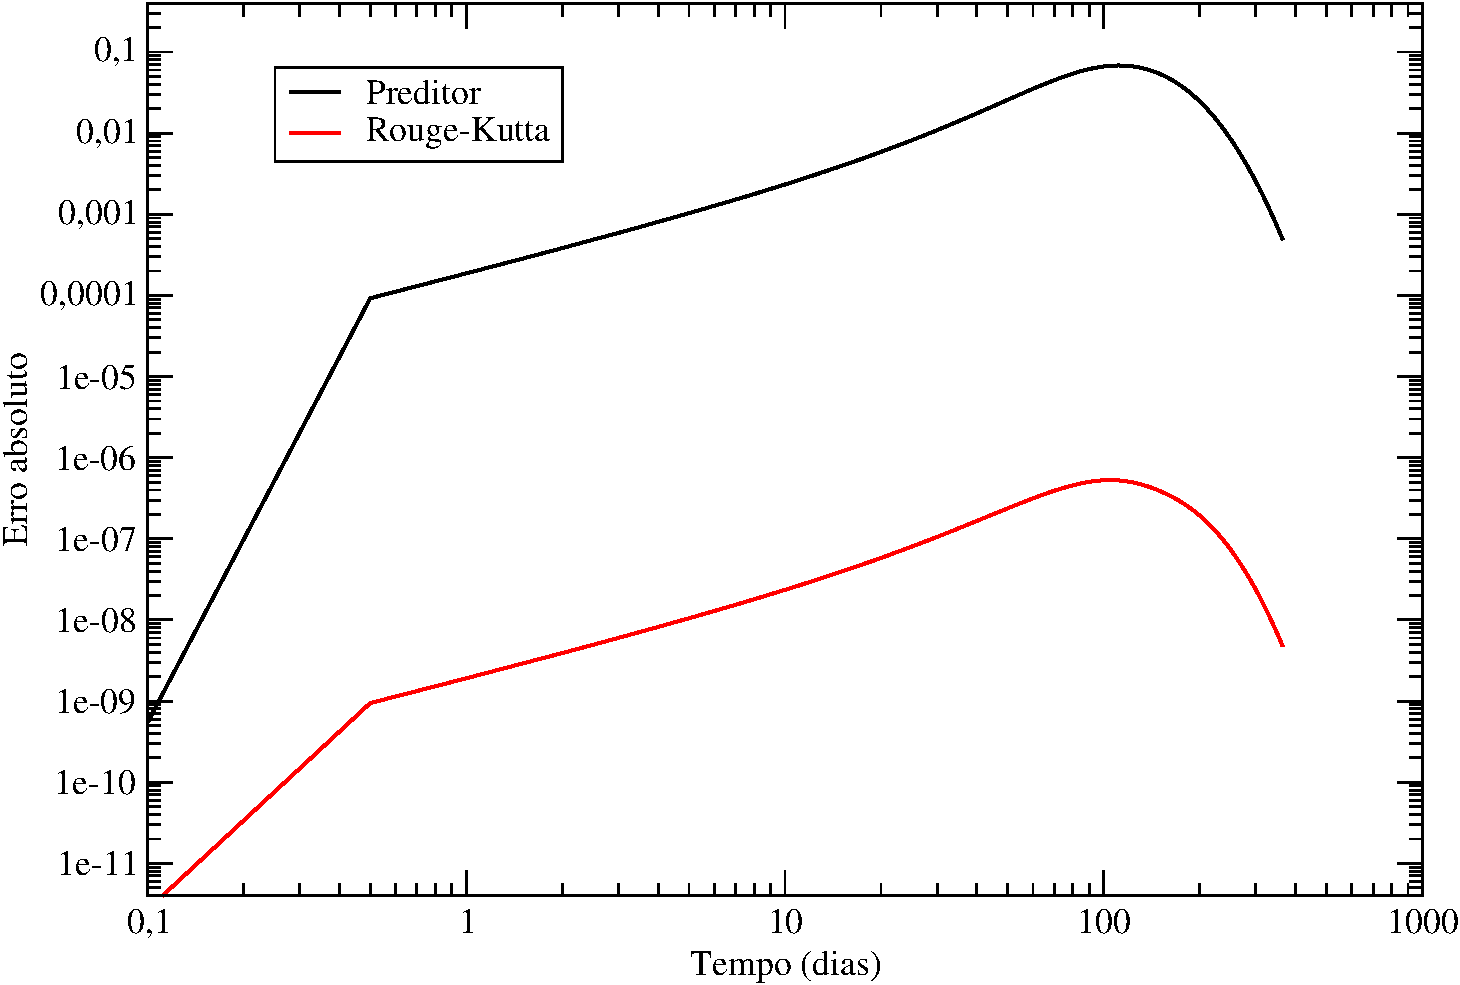
\includegraphics[width=0.447\textwidth]{1errork.pdf}
\caption{Erro absoluto para o método de Corretor-Preditor e Rouge-Kutta de quarta ordem para N = 730.}
\label{errork}
\end{figure}

\subsection*{ d) }
Na figura \ref{popfinal} estão representadas as populações para os três parâmetros pedidos. A curva preta mostra uma população que satura perto dos 4000 indivíduos;  a curva vermelha mostra uma população que, apesar de decrescente, satura em um valor também próximo de 4000 indivíduos. A saturação está relacionada ao parâmetro $\kappa$, como pode ser visto aplicando o limite de tempos longos na equação do número de indivíduos.  A curva azul, no entanto, possui uma taxa de crescimento de população negativa e mostra uma população cujo número final de indivíduos vai para zero, mesmo tendo o mesmo valor de $\kappa$ das outras curvas.
\begin{figure}
\centering
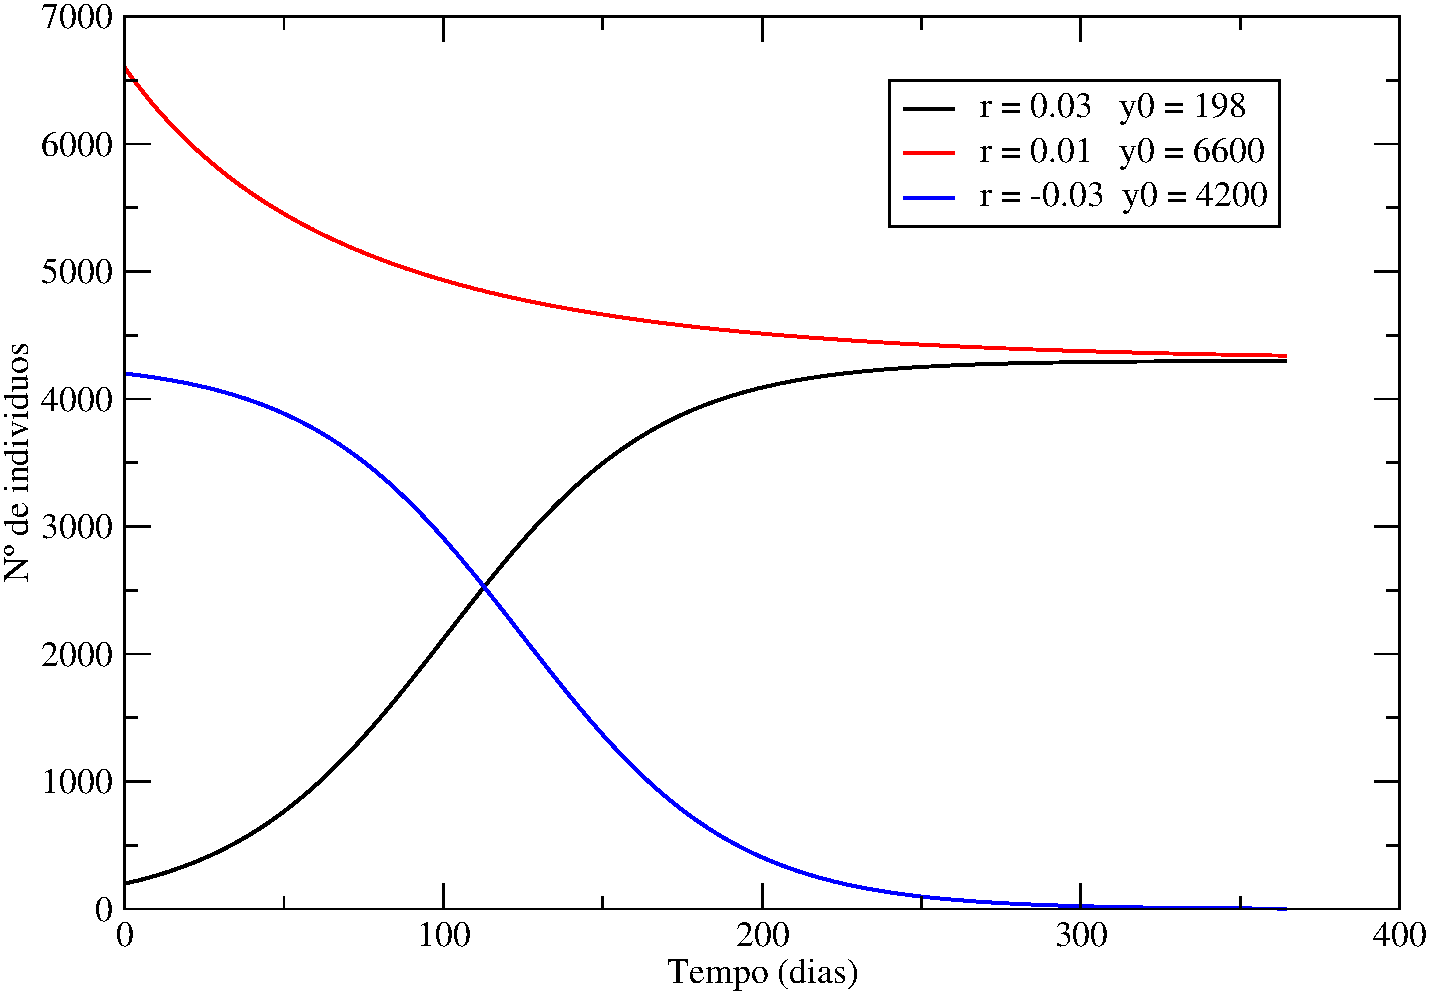
\includegraphics[width=0.447\textwidth]{1final.pdf}
\caption{População em função do tempo para três conjuntos de parâmetros.}
\label{popfinal}
\end{figure}


\section*{Exercício 2}

\subsection*{a)}
Os resultados estão na figura \ref{pop}. No gráfico da esquerda temos a evolução temporal das três populações, onde vemos que após um tempo t = 300 há uma convergência no valor de cada uma delas. Na figura à direita os três valores teóricos para o estado estacionário foram plotados como linhas horizontais, de modo que a comparação com o valor teórico é imediata em qualquer ponto. Note que a solução estacionária não é válida para tempos curtos, passando a ser válida somente para tempos t $>$ 350.



\begin{figure}[!htb]
\centering
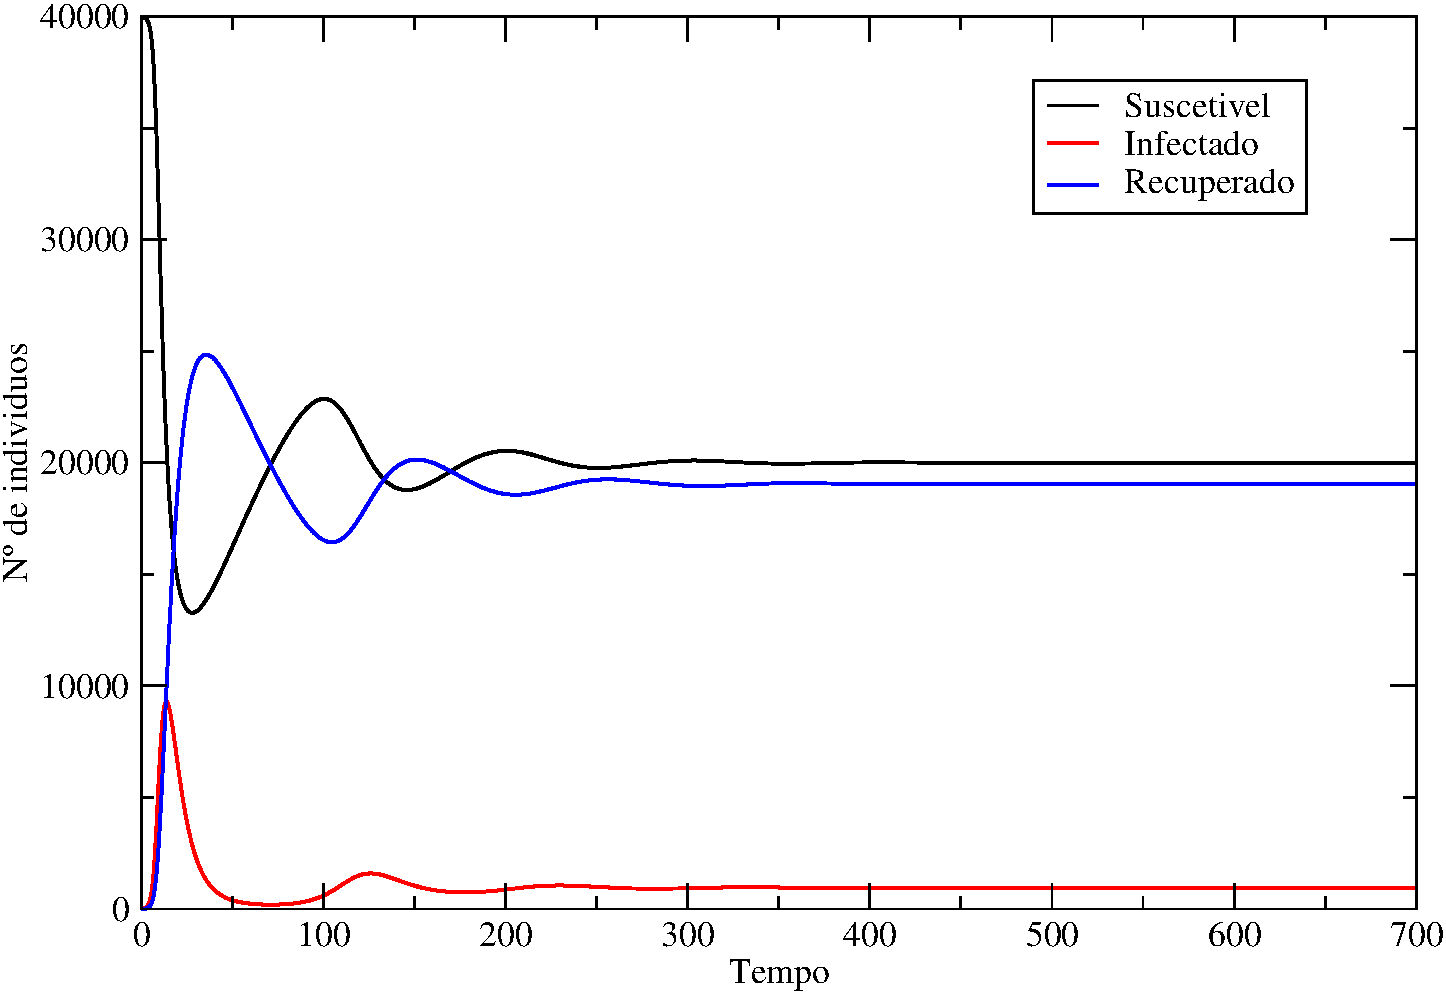
\includegraphics[width=0.447\textwidth]{2graph.pdf}
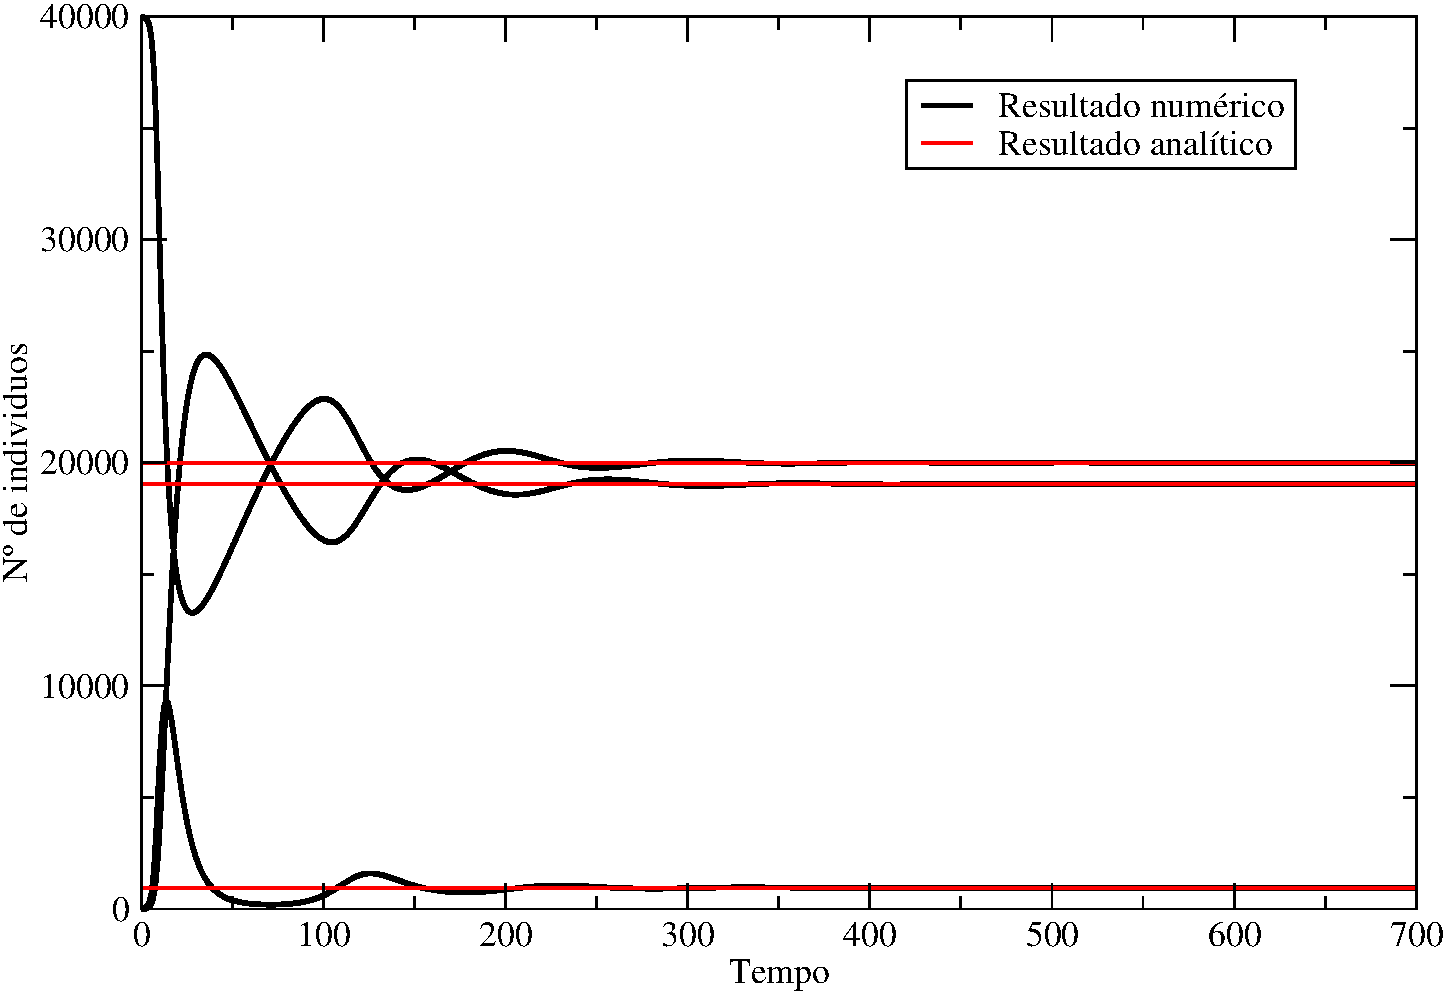
\includegraphics[width=0.447\textwidth]{2erro.pdf}
\caption{População de Suscetiveis, Infectados e Recuperados em função do tempo.}
\label{pop}
\end{figure}





\section*{Exercício 3}
\subsection*{a)}
Temos que o potencial é dado por:

\begin{equation*}
V(r) = -D \left[ 	1 	- \left(		1	-	\mathrm{e}^{-a(r-r_e)} \right) ^2 \right]
\end{equation*}
\label{V}

Derivando em função de r e multiplicando por -1 temos a expressão para a força:

\begin{equation*}
F(r) = -aD \left[ 	1 	- 2\left(		1	-	\mathrm{e}^{-a(r-r_e)} \right) \mathrm{e}^{-a(r-r_e)} \right]
\end{equation*}
\label{F}

Na figura \ref{VeF} foi feito o gráfico do potencial e da força em função da posição. Além disso, foi feito também a força em uma região próxima do mínimo de potencial, de modo a evidenciar o comportamento linear da força próximo nesta região.

\begin{figure}[!t]
\centering
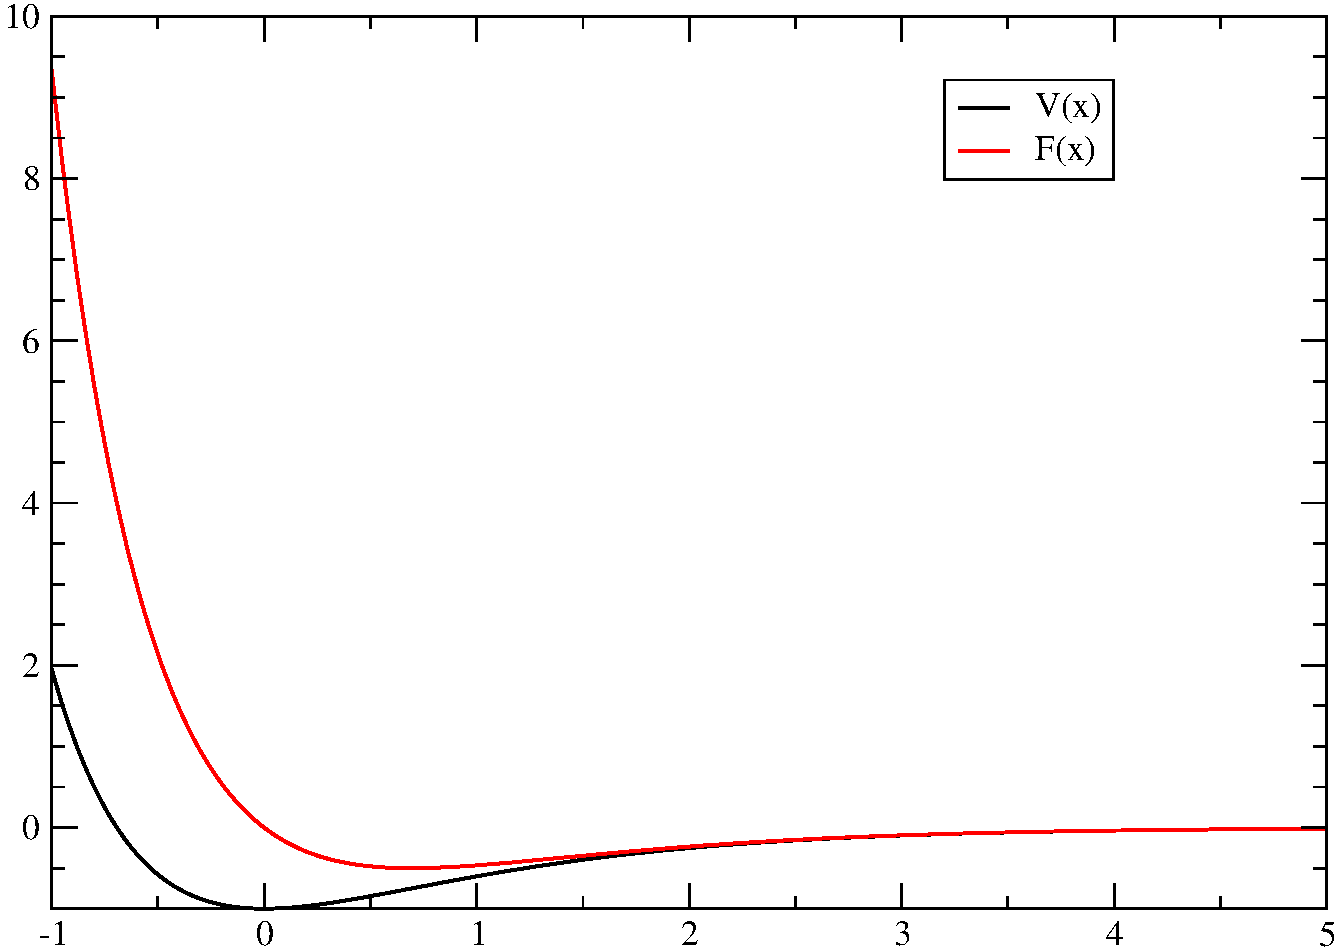
\includegraphics[width=0.447\textwidth]{potential.pdf}
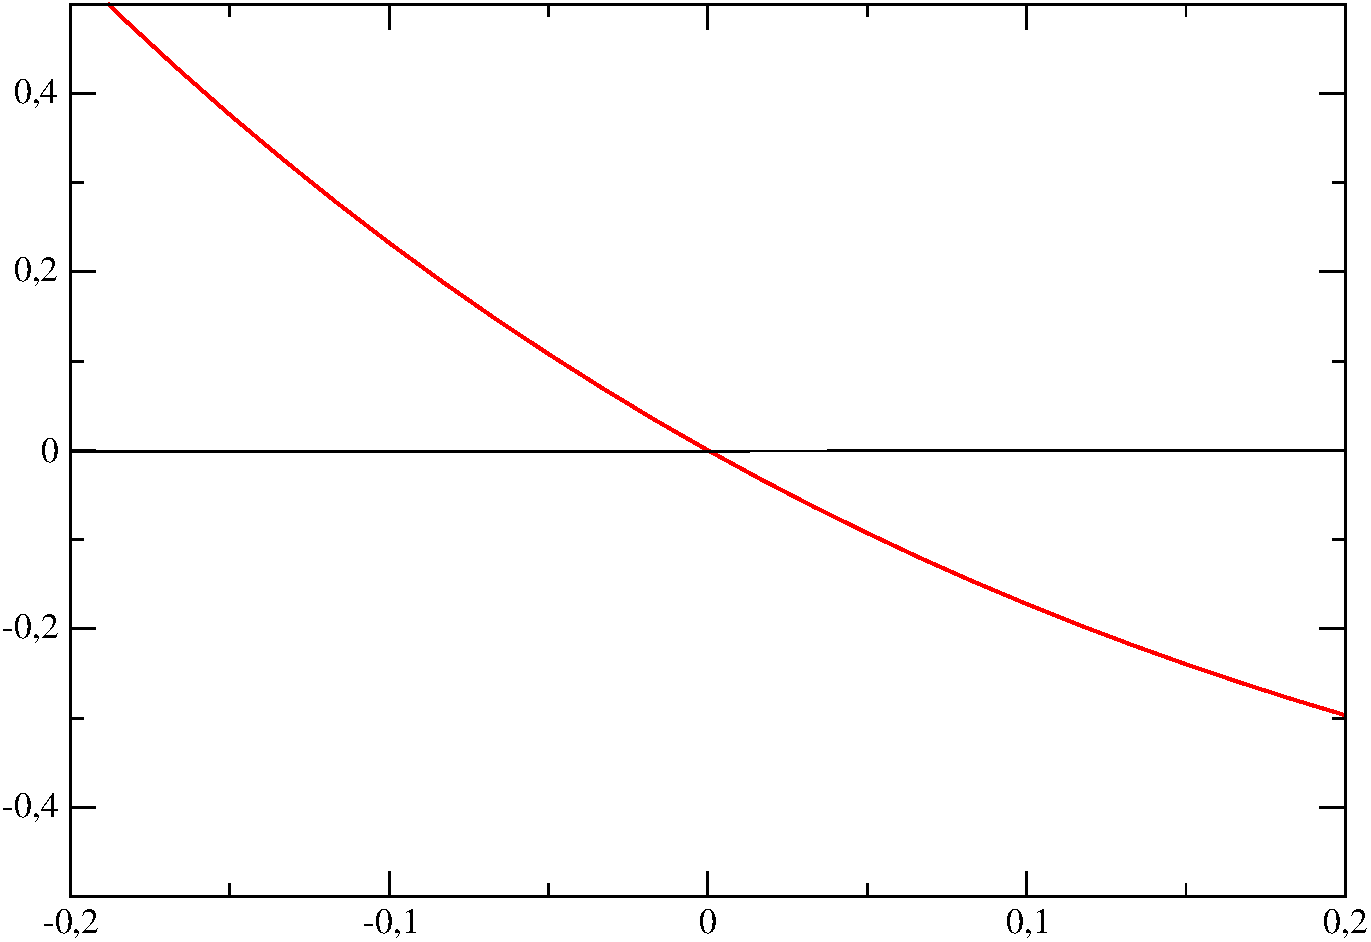
\includegraphics[width=0.447\textwidth]{zoom.pdf}
\caption{Potencial e Força em função da posição (esquerda) e força em pontos próximos do mínimo de potencial (direita).}
\label{VeF}
\end{figure}

\subsection*{b)}

Para calcular o valor teórico precisamos do valor de $\delta$. Fazendo $s(t_0) = 1$ temos:
\begin{equation*}
\delta =  \arccos \left[ \left(\frac{E+D}{D} \right)^\frac{1}{2} \right]  
\end{equation*}
\label{F}

Na figura \ref{xev} temos a posição em função do tempo calculada numericamente e exatamente à esquerda e o valor do erro absoluto à direita. Na figura \ref{xeverro} temos a posição e a velocidade em função do tempo obtidas numéricamente.

\begin{figure}[!htb]
\centering
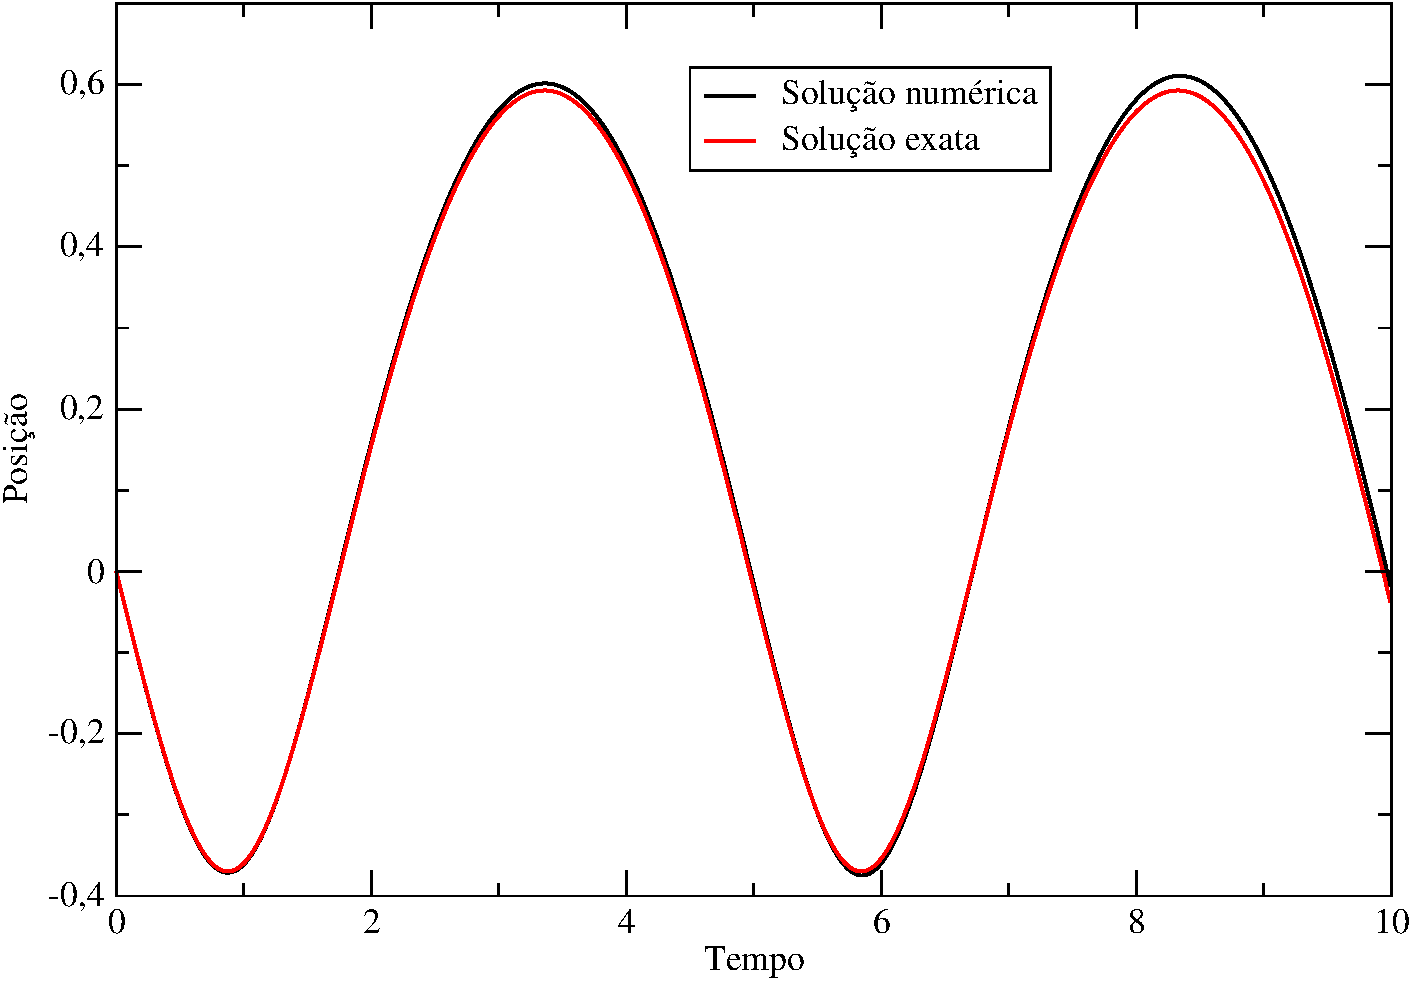
\includegraphics[width=0.447\textwidth]{exata.pdf}
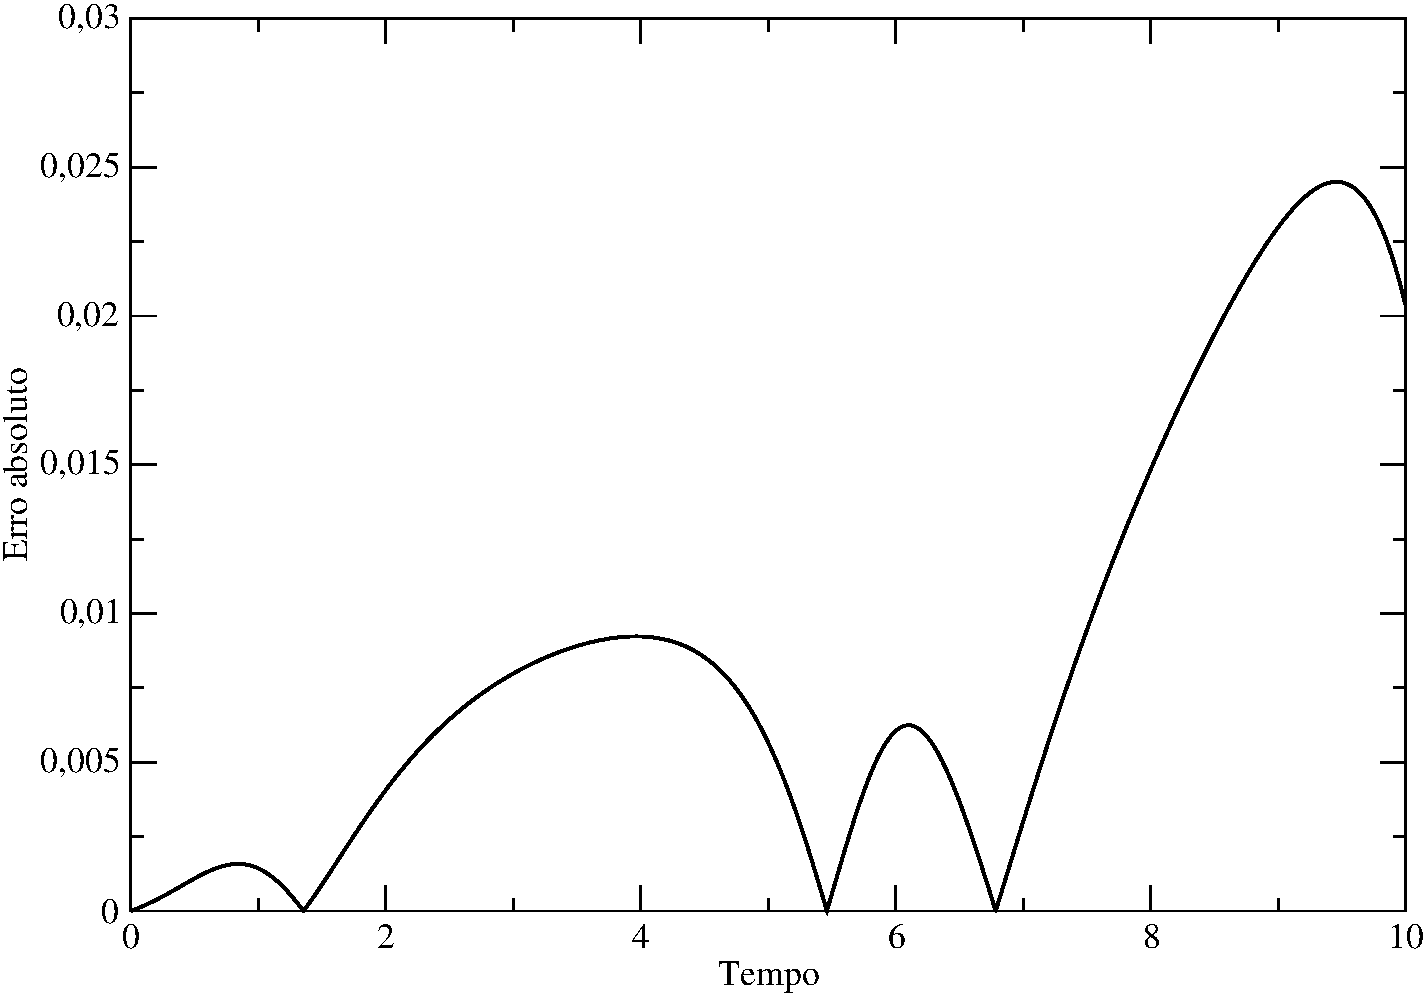
\includegraphics[width=0.447\textwidth]{3erro.pdf}
\caption{Posição e velocidade em função do tempo (esquerda) e erro absoluto da posição (direita).}
\label{xev}
\end{figure}

\begin{figure}[!tb]
\centering
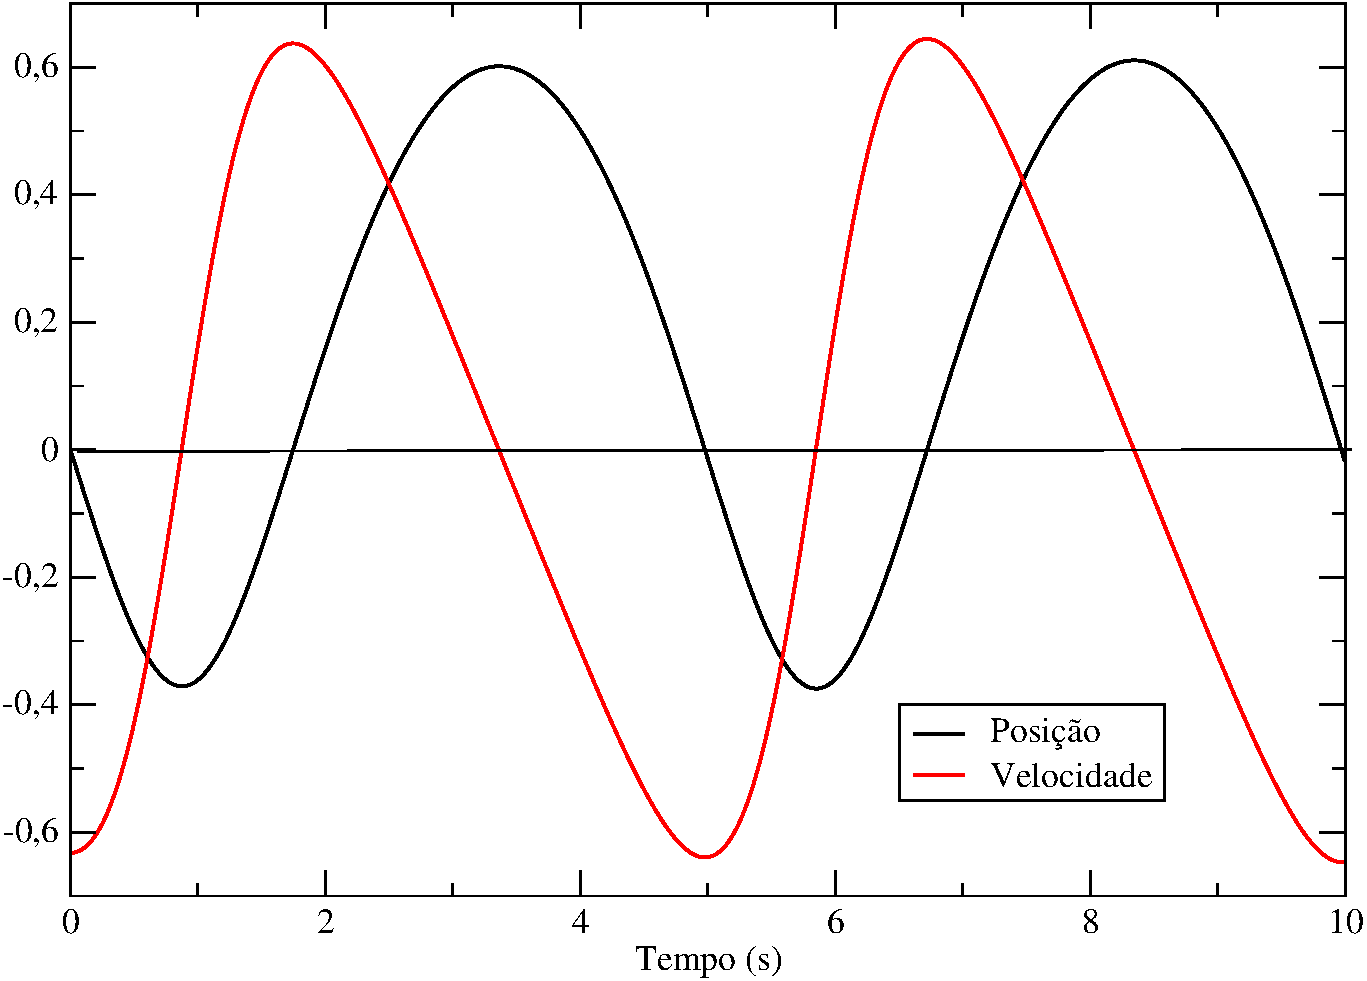
\includegraphics[width=0.447\textwidth]{xev.pdf}
\caption{Comparação entre solução numérica e exata.}
\label{xeverro}
\end{figure}






\section*{Exercício 4}
\subsection*{a)}

A EDO $\nabla^2 u(x) = 0 $ possui como solução exata $u(x) = C_1 x + C_2 $. Aplicando as condições de contorno $u(0) = 305K$ e $u(30) = 390K$, temos $u(x) = 2.833 x + 305 $. Na figura \ref{u} temos a temperatura em função da posição calculada numericamente e o erro absoluto associado.

\begin{figure}[!b]
\centering
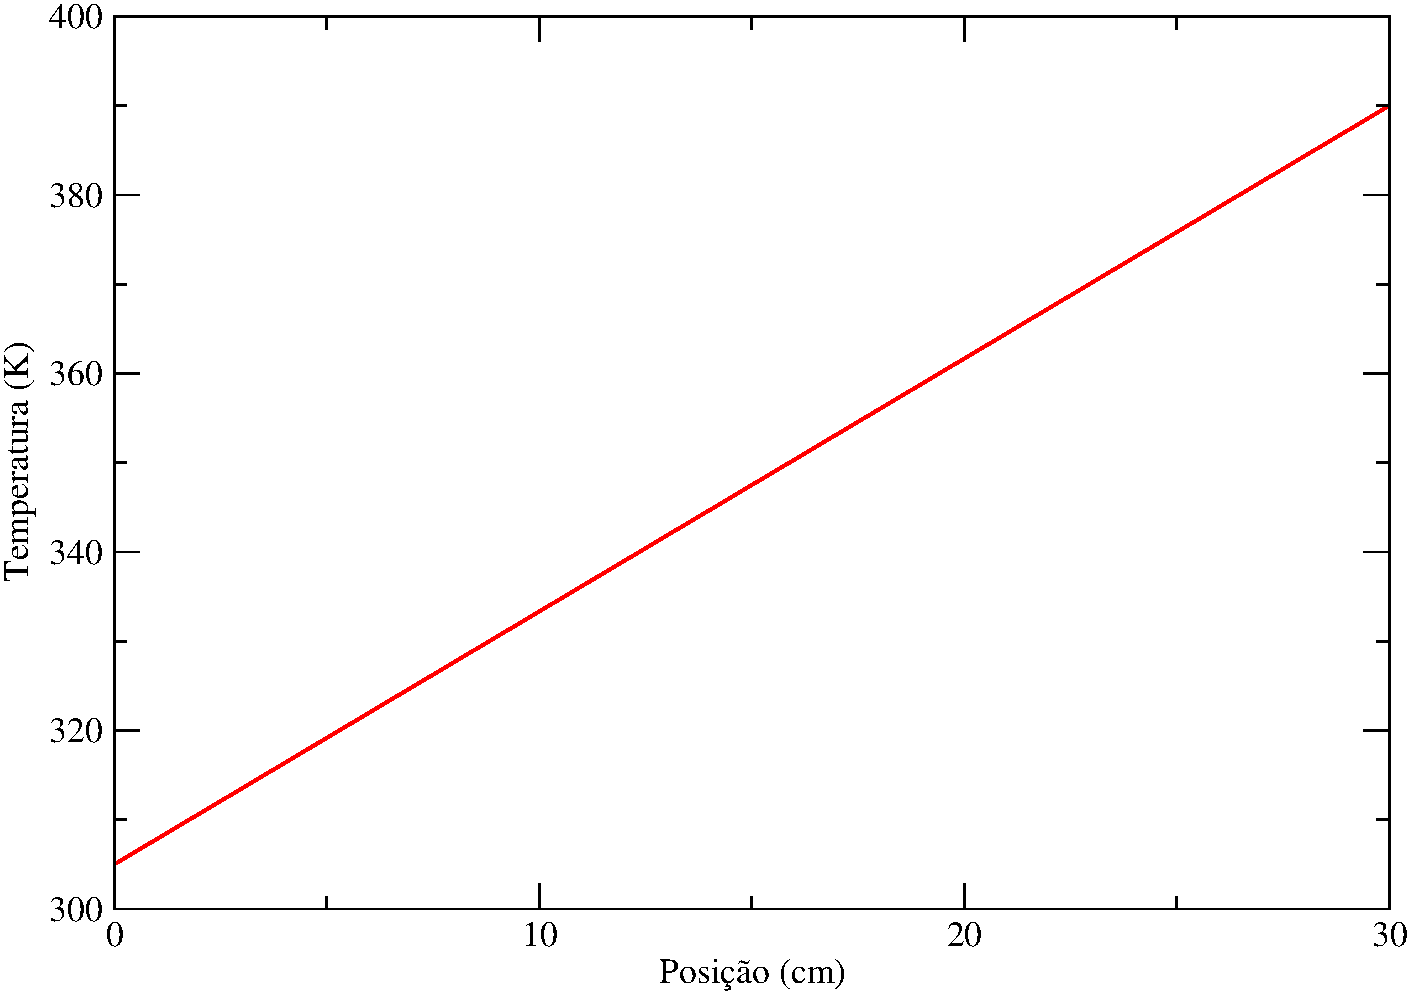
\includegraphics[width=0.447\textwidth]{u.pdf}
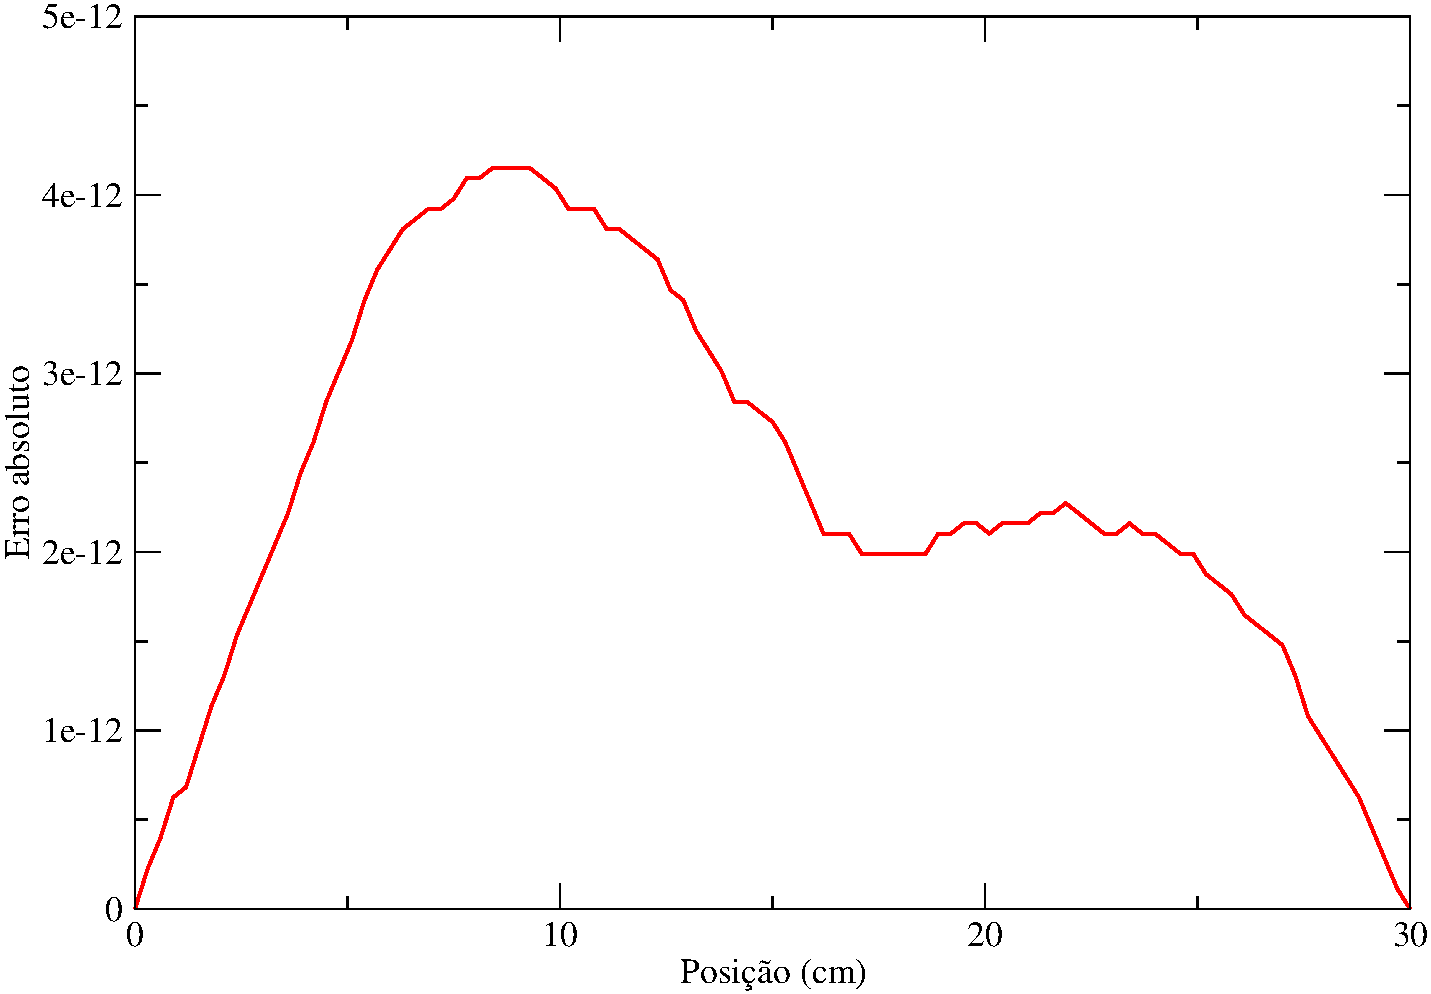
\includegraphics[width=0.447\textwidth]{erro.pdf}
\caption{Temperatura em função da posição (esquerda) e erro absoluto em função da posição (direita).}
\label{u}
\end{figure}


\subsection*{b)}

As novas condições de contorno são dadas por:


$\begin{cases} 
u(0) = 305 K \\ 
\frac{\partial u}{\partial x} \Big|_{x=30} = -4 K/cm
\end{cases} $
\vspace{3pt}


Comparando com as equações dadas:

\vspace{3pt}

$\begin{cases} 
\alpha_L u(x) + \beta_L \frac{\partial u}{\partial x} = \gamma_L \\ 
\alpha_H u(x) + \beta_H \frac{\partial u}{\partial x} = \gamma_H
\end{cases} $

\vspace{3pt}

Temos que 
$\begin{cases} 
\beta_L = 0 \\ 
\alpha_H = 0
\end{cases} $


Se escolhermos, por conveniência, que
$\begin{cases} 
\alpha_L = 1 \\ 
\beta_H = 1
\end{cases} $

Temos finalmente que
$\begin{cases} 
\gamma_L = 305 \\ 
\gamma_H = -4
\end{cases} $

Com isto, pelo algoritmo da referência [4] temos que a matriz M será modificada apenas na ultima linha, onde o elemento da diagonal passa de -2 para -1. A matriz w também será alterada apenas na ultima linha, onde $w(N) = f(x) (dx)^2 + 4 dx$. No entanto houve algum erro na implementação, pois o resultado obtido está longe do resultado teórico esperado, como pode ser visto na figura \ref{ultimo}.


\begin{figure}[!t]
\centering
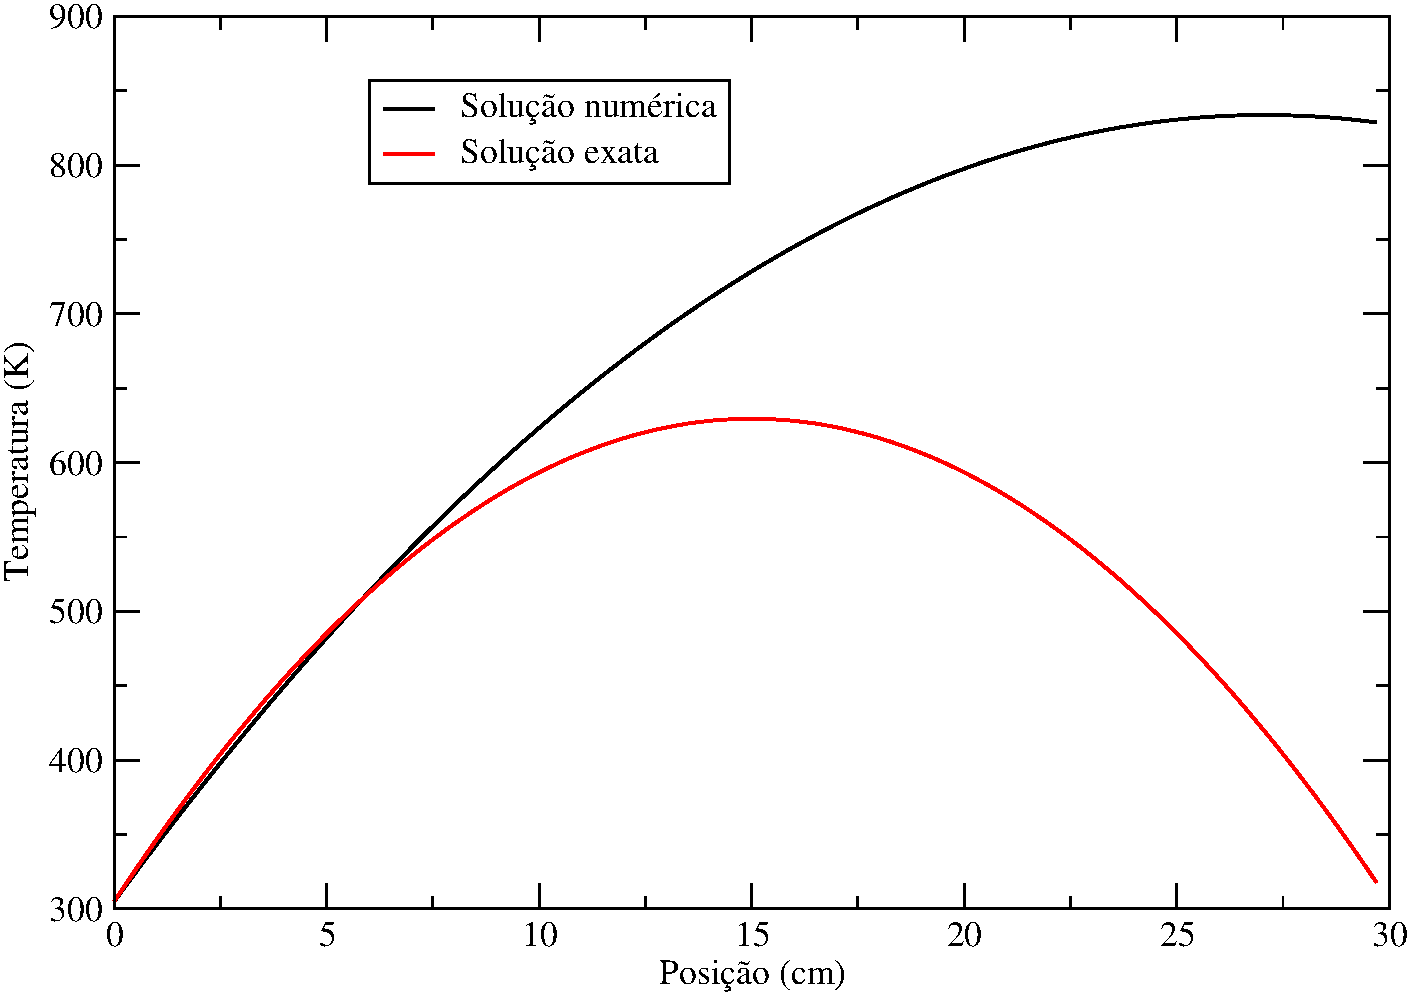
\includegraphics[width=0.447\textwidth]{g.pdf}
\caption{Comparação entre solução numérica e exata.}
\label{ultimo}
\end{figure}


\end{document}
